%-----------------------------------------------------------------------------%
\chapter{\babEmpat}
%-----------------------------------------------------------------------------%
%-----------------------------------------------------------------------------%
\section{Membuat Tabel}
%-----------------------------------------------------------------------------%

\begin{figure}
	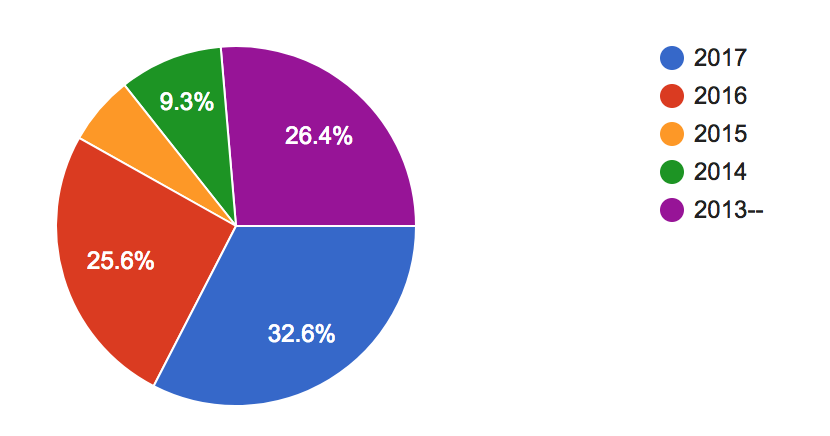
\includegraphics{pics/angkatan}
	\caption{Alur tahapan penelitian}
	\centering
\end{figure}
\begin{figure}
	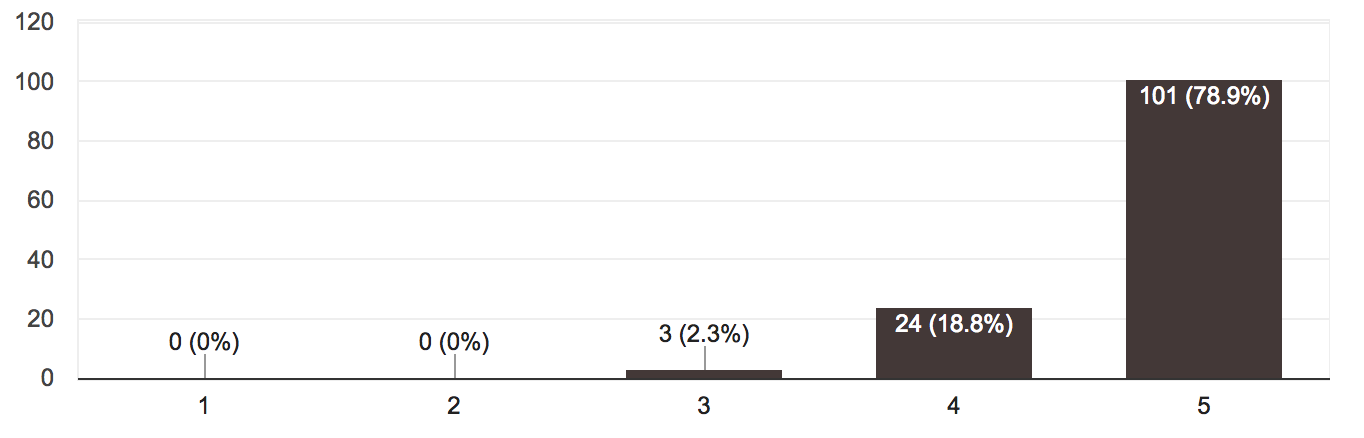
\includegraphics[width=\linewidth]{pics/contoh-langsung}
	\caption{Alur tahapan penelitian}
	\centering
\end{figure}
\begin{figure}
	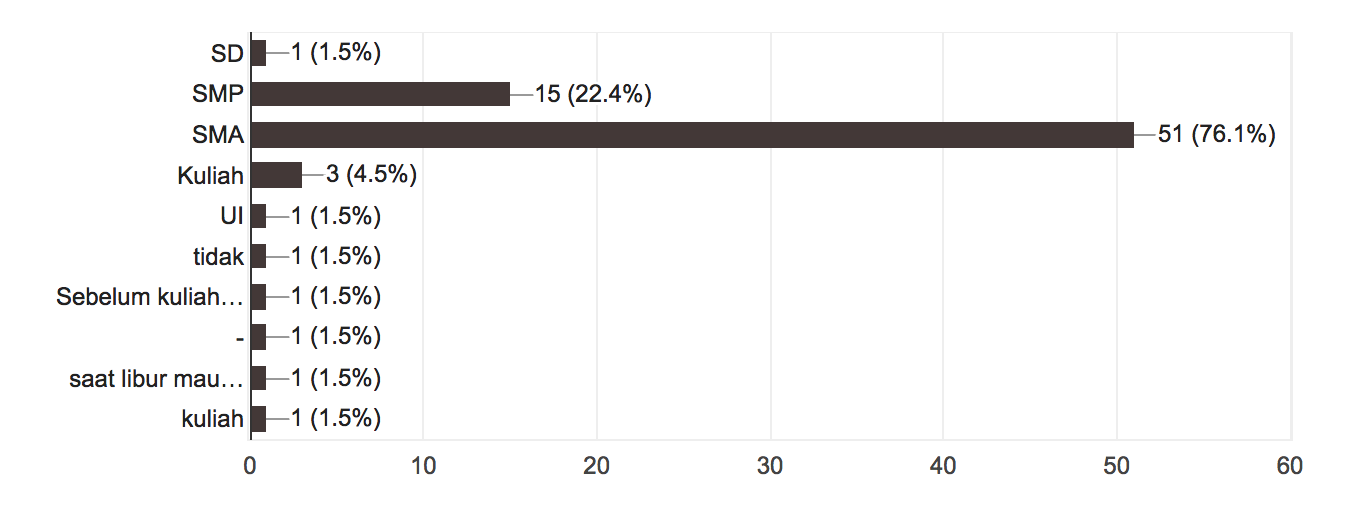
\includegraphics[width=\linewidth]{pics/kapan-pernah-belajarnya}
	\caption{Alur tahapan penelitian}
	\centering
\end{figure}
\begin{figure}
	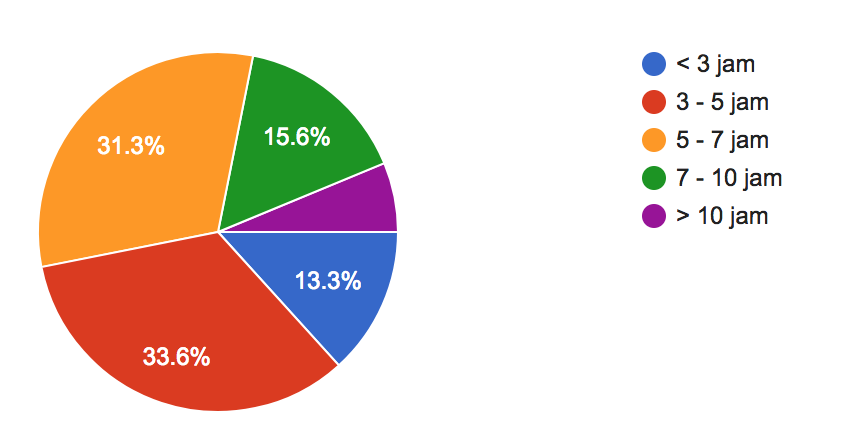
\includegraphics[width=\linewidth]{pics/lama-belajar}
	\caption{Alur tahapan penelitian}
	\centering
\end{figure}
\begin{figure}
	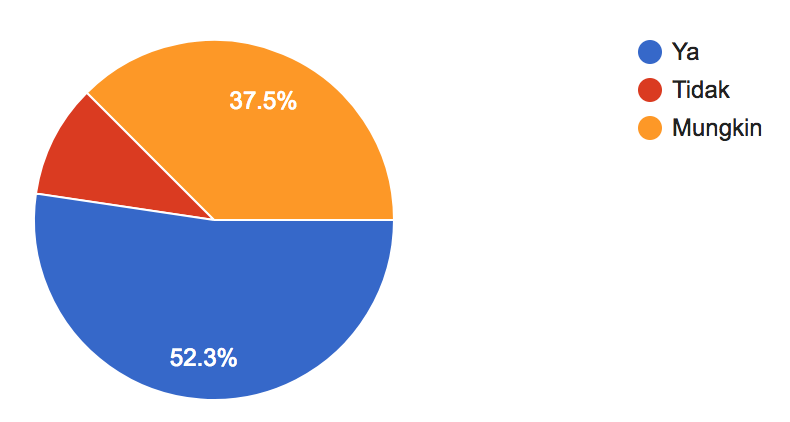
\includegraphics[width=\linewidth]{pics/lebih-senang-bermain-game}
	\caption{Alur tahapan penelitian}
	\centering
\end{figure}
\begin{figure}
	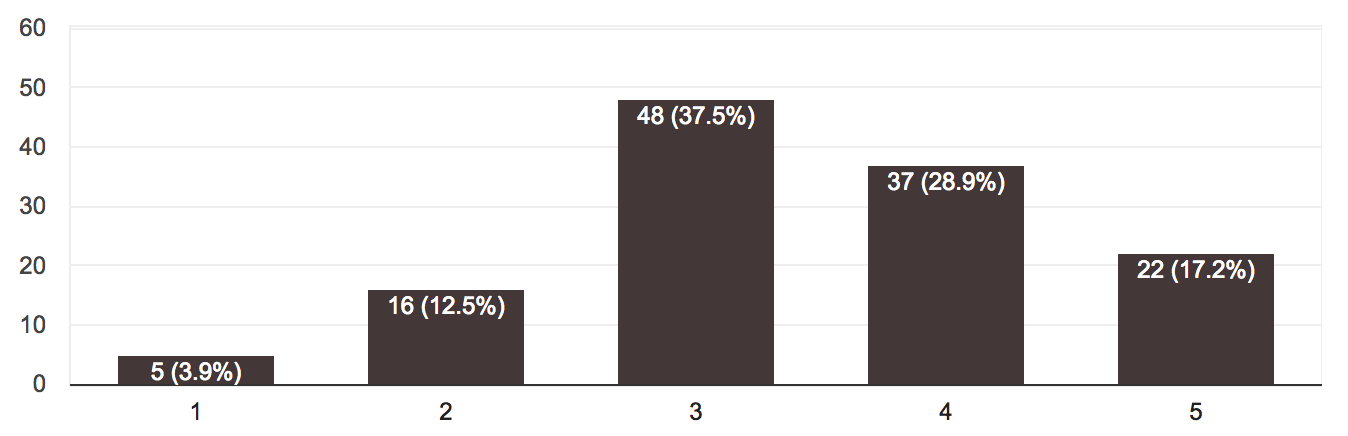
\includegraphics[width=\linewidth]{pics/menggali-lebih-dalam-sendiri}
	\caption{Alur tahapan penelitian}
	\centering
\end{figure}
\begin{figure}
	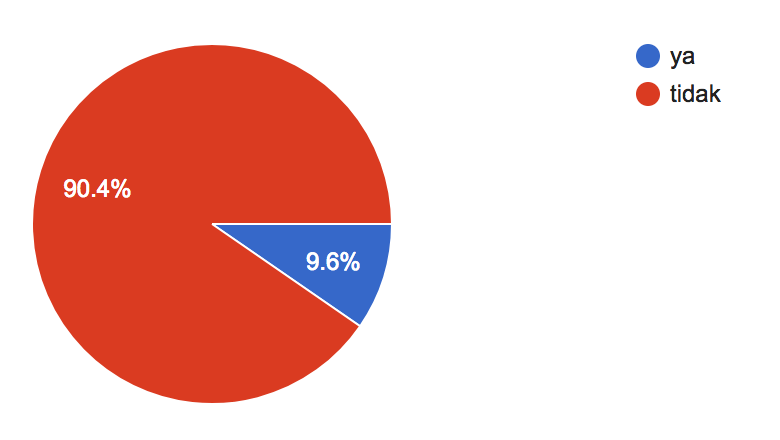
\includegraphics[width=\linewidth]{pics/mengulang-ddp}
	\caption{Alur tahapan penelitian}
	\centering
\end{figure}
\begin{figure}
	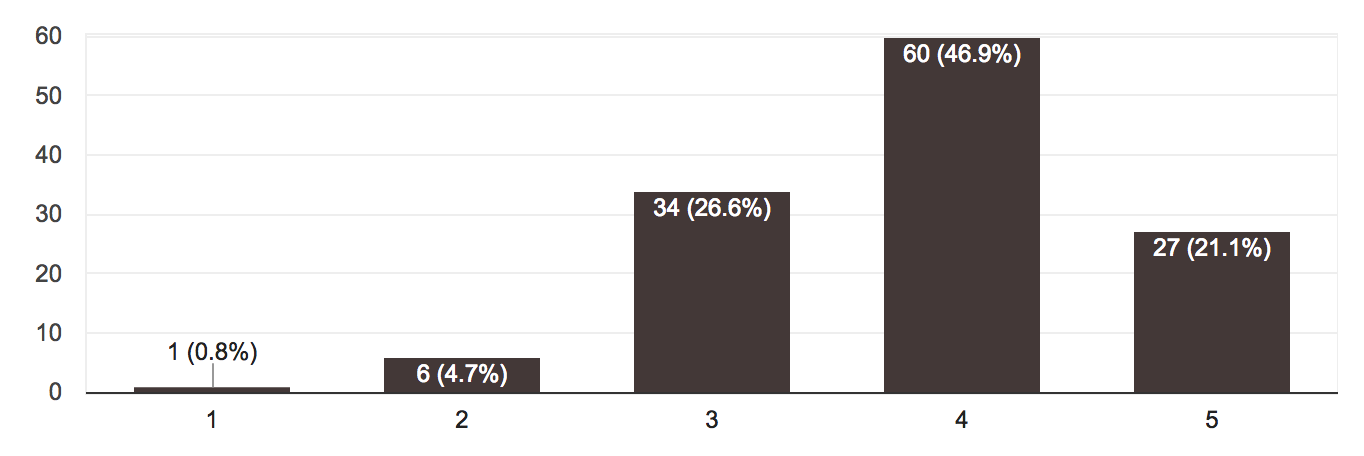
\includegraphics[width=\linewidth]{pics/menikmati-cara-belajar-sekarang}
	\caption{Alur tahapan penelitian}
	\centering
\end{figure}
\begin{figure}
	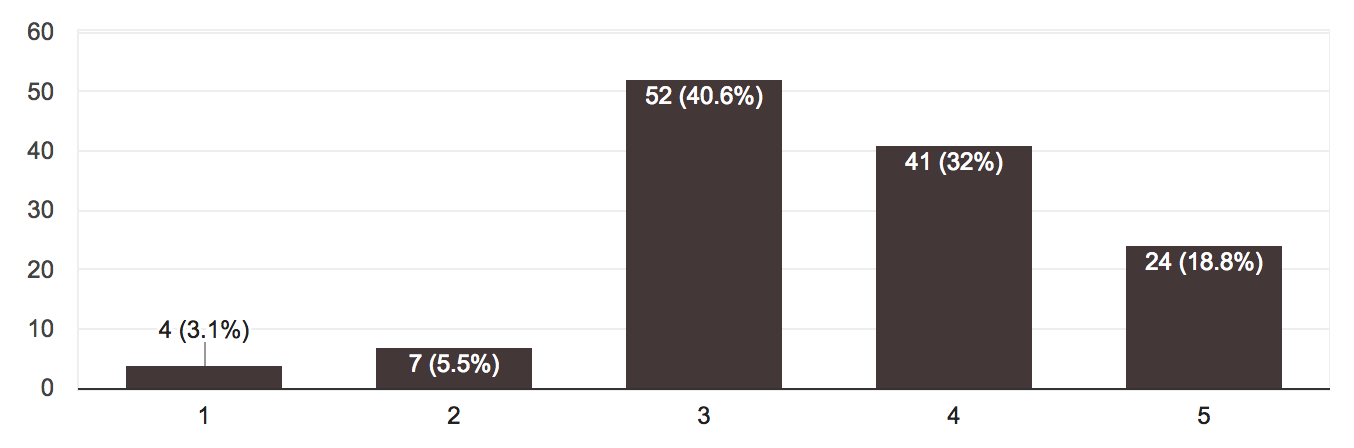
\includegraphics[width=\linewidth]{pics/mudah-memahami}
	\caption{Alur tahapan penelitian}
	\centering
\end{figure}
\begin{figure}
	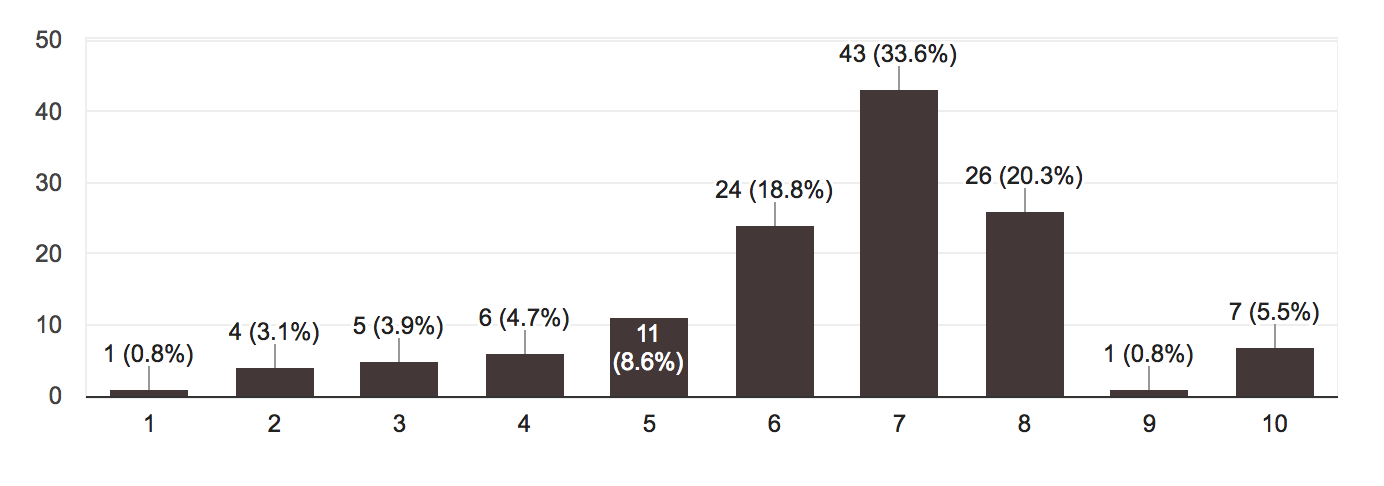
\includegraphics[width=\linewidth]{pics/nilai-pemograman}
	\caption{Alur tahapan penelitian}
	\centering
\end{figure}
\begin{figure}
	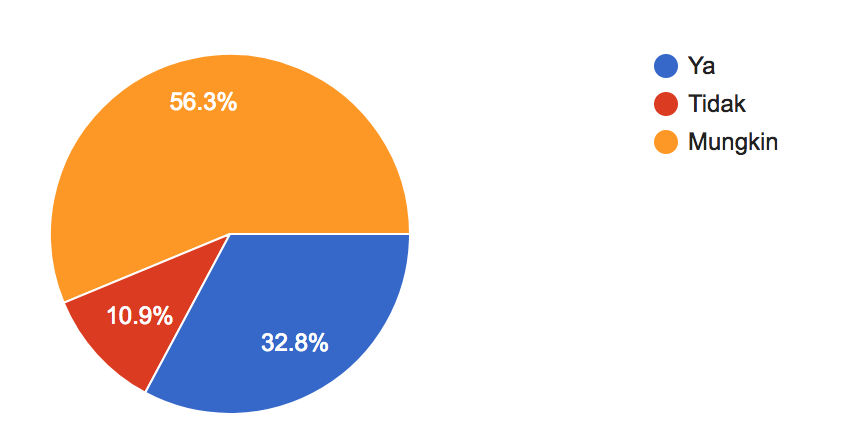
\includegraphics[width=\linewidth]{pics/passion-pemograman}
	\caption{Alur tahapan penelitian}
	\centering
\end{figure}
\begin{figure}
	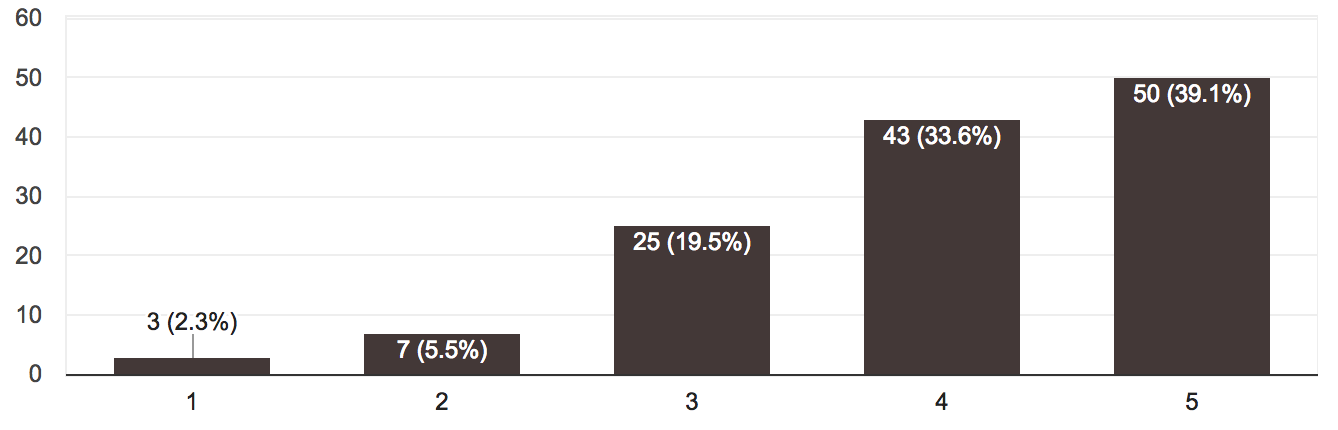
\includegraphics[width=\linewidth]{pics/perlu-waktu-luar-kelas}
	\caption{Alur tahapan penelitian}
	\centering
\end{figure}
\begin{figure}
	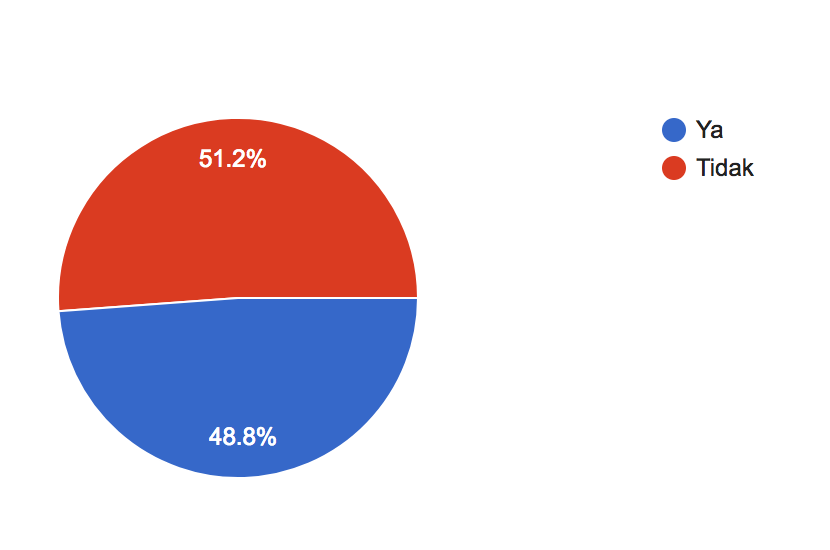
\includegraphics[width=\linewidth]{pics/pernah-ikut-ddp-sebelum}
	\caption{Alur tahapan penelitian}
	\centering
\end{figure}
\begin{figure}
	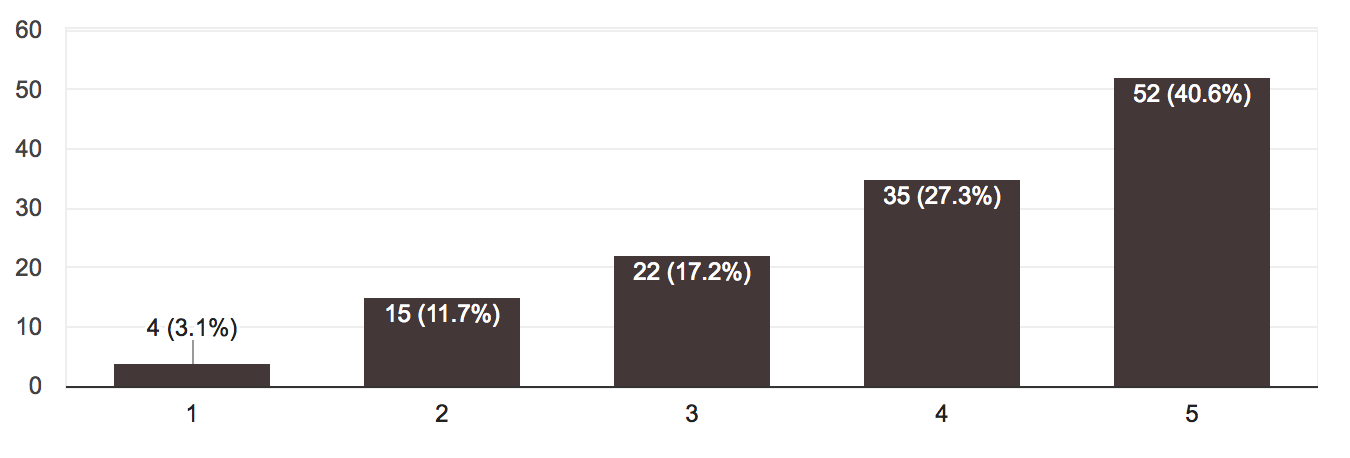
\includegraphics[width=\linewidth]{pics/slide-show-x-buku}
	\caption{Alur tahapan penelitian}
	\centering
\end{figure}
\begin{figure}
	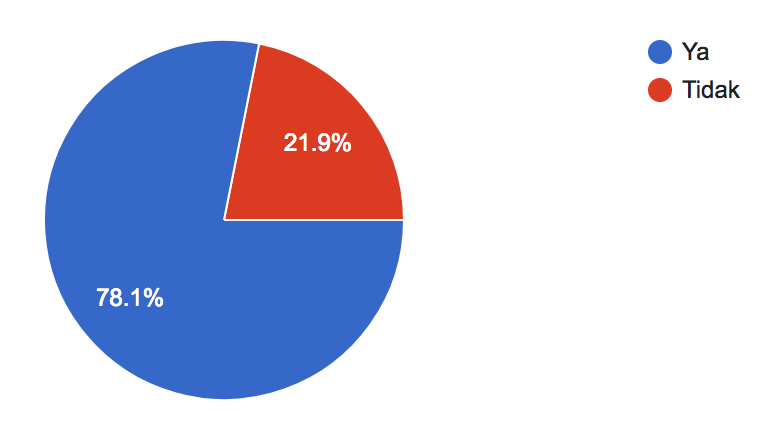
\includegraphics[width=\linewidth]{pics/suka-bermain-game}
	\caption{Alur tahapan penelitian}
	\centering
\end{figure}
\begin{figure}
	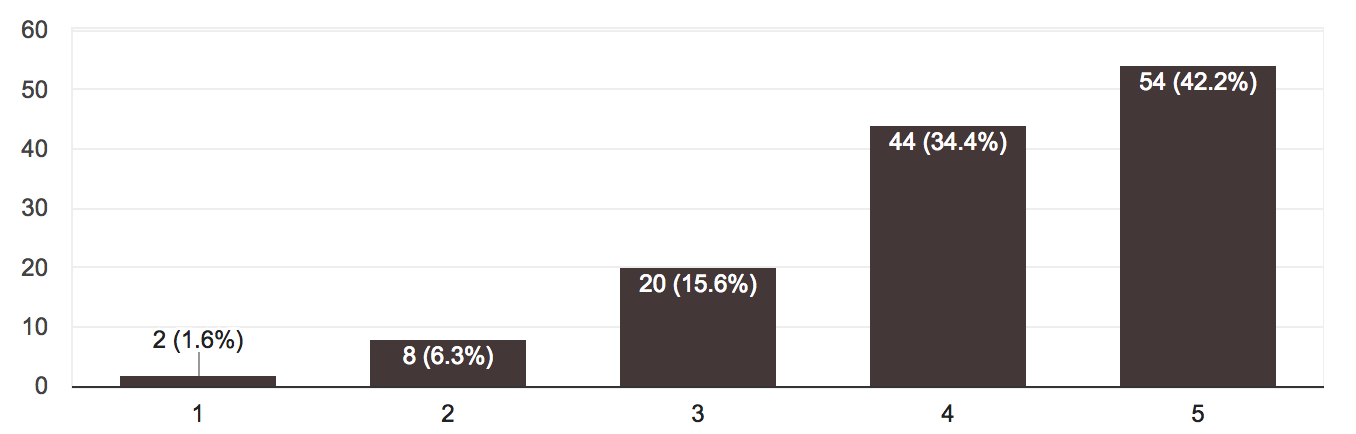
\includegraphics[width=\linewidth]{pics/tidak-suka-teori-saja}
	\caption{Alur tahapan penelitian}
	\centering
\end{figure}
\begin{figure}
	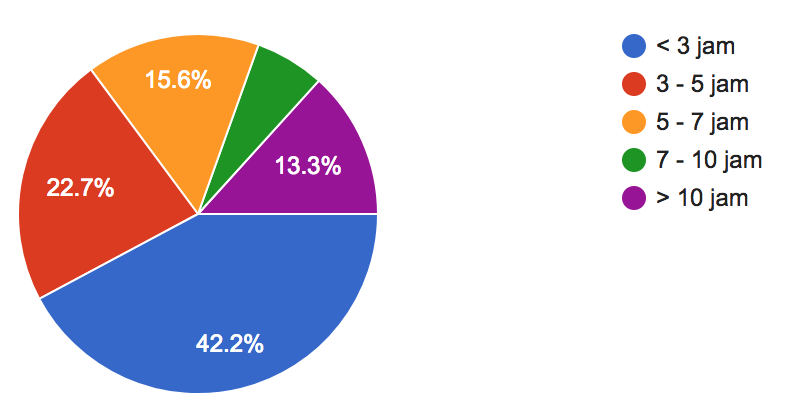
\includegraphics[width=\linewidth]{pics/waktu-bermain-game}
	\caption{Alur tahapan penelitian}
	\centering
\end{figure}

\begin{table}
	\centering
	\caption{Contoh Tabel}
	\label{tab:tab1}
	\begin{tabular}{| l | c r |}
		\hline
		& kol 1 & kol 2 \\ 
		\hline
		baris 1 & 1 & 2 \\
		baris 2 & 3 & 4 \\
		baris 3 & 5 & 6 \\
		jumlah  & 9 & 12 \\
		\hline
	\end{tabular}
\end{table}

Ada jenis tabel lain yang dapat dibuat dengan \latex~berikut 
beberapa diantaranya. 
Contoh-contoh ini bersumber dari 
\url{http://en.wikibooks.org/wiki/LaTeX/Tables}

\begin{table}
	\centering
	\caption{An Example of Rows Spanning Multiple Columns}
	\label{row.spanning}
	\begin{tabular}{|l|l|*{6}{c|}}
  		\hline % create horizontal line
  		No & Name & \multicolumn{3}{|c|}{Week 1} & \multicolumn{3}{|c|}{Week 2} \\
  		\cline{3-8} % create line from 3rd column till 8th column
  		& & A & B & C & A & B & C\\
  		\hline
  		1 & Lala & 1 & 2 & 3 & 4 & 5 & 6\\
  		2 & Lili & 1 & 2 & 3 & 4 & 5 & 6\\
  		3 & Lulu & 1 & 2 & 3 & 4 & 5 & 6\\
  		\hline
	\end{tabular}
\end{table}

\begin{table}
	\centering
	\caption{An Example of Columns Spanning Multiple Rows}
	\label{column.spanning}
	\begin{tabular}{|l|c|l|}
		\hline
		Percobaan & Iterasi & Waktu \\
		\hline
		Pertama & 1 & 0.1 sec \\ \hline
		\multirow{2}{*}{Kedua} & 1 & 0.1 sec \\
 		& 3 & 0.15 sec \\ 
 		\hline
		\multirow{3}{*}{Ketiga} & 1 & 0.09 sec \\
 		& 2 & 0.16 sec \\
 		& 3 & 0.21 sec \\ 
 		\hline
	\end{tabular}
\end{table}

\begin{table}
	\centering
	\caption{An Example of Spanning in Both Directions Simultaneously}
	\label{mix.spanning}
	\begin{tabular}{cc|c|c|c|c|}
		\cline{3-6}
		& & \multicolumn{4}{|c|}{Title} \\ \cline{3-6}
		& & A & B & C & D \\ \hline
		\multicolumn{1}{|c|}{\multirow{2}{*}{Type}} &
		\multicolumn{1}{|c|}{X} & 1 & 2 & 3 & 4\\ \cline{2-6}
		\multicolumn{1}{|c|}{}                        &
		\multicolumn{1}{|c|}{Y} & 0.5 & 1.0 & 1.5 & 2.0\\ \cline{1-6}
		\multicolumn{1}{|c|}{\multirow{2}{*}{Resource}} &
		\multicolumn{1}{|c|}{I} & 10 & 20 & 30 & 40\\ \cline{2-6}
		\multicolumn{1}{|c|}{}                        &
		\multicolumn{1}{|c|}{J} & 5 & 10 & 15 & 20\\ \cline{1-6}
	\end{tabular}
\end{table}

%-----------------------------------------------------------------------------%
\section{thesis.tex}
%-----------------------------------------------------------------------------%
Berkas ini berisi seluruh berkas Latex yang dibaca, jadi bisa dikatakan sebagai 
berkas utama. Dari berkas ini kita dapat mengatur bab apa saja yang ingin 
kita tampilkan dalam dokumen.


%-----------------------------------------------------------------------------%
\section{laporan\_setting.tex}
%-----------------------------------------------------------------------------%
Berkas ini berguna untuk mempermudah pembuatan beberapa template standar. 
Anda diminta untuk menuliskan judul laporan, nama, npm, dan hal-hal lain yang 
dibutuhkan untuk pembuatan template. 


%-----------------------------------------------------------------------------%
\section{istilah.tex}
%-----------------------------------------------------------------------------%
Berkas istilah digunakan untuk mencatat istilah-istilah yang digunakan. 
Fungsinya hanya untuk memudahkan penulisan.
Pada beberapa kasus, ada kata-kata yang harus selalu muncul dengan tercetak 
miring atau tercetak tebal. 
Dengan menjadikan kata-kata tersebut sebagai sebuah perintah \latex~tentu akan 
mempercepat dan mempermudah pengerjaan laporan. 


%-----------------------------------------------------------------------------%
\section{hype.indonesia.tex}
%-----------------------------------------------------------------------------%
Berkas ini berisi cara pemenggalan beberapa kata dalam bahasa Indonesia. 
\latex~memiliki algoritma untuk memenggal kata-kata sendiri, namun untuk 
beberapa kasus algoritma ini memenggal dengan cara yang salah. 
Untuk memperbaiki pemenggalan yang salah inilah cara pemenggalan yang benar 
ditulis dalam berkas hype.indonesia.tex.